\section{}

We use the following stochastic process as our data generation model for the time dependent variable $y_t$ in an arbitrary time step $t\in[1,T]$.
Note that, except for the $y_t$'s, all of the following are random variables generated by parametric distributions defined by our model.
The stochastic process is modelled as follows:
\begin{align}
    \nonumber&\mathbf{z}_{1} =  \mathbf{s}_0\\
    \nonumber&y_1 =  \mathbf{x}_1 {}^\intercal  \mathbf{z}_1\\
    \nonumber&\mathbf{z}_{2} =  \mathbf{Z}_2^*{}\cdot \mathbf{z}_1 \\
    \nonumber&y_2 = \mathbf{x}_2 {}^\intercal \mathbf{z}_2 \\
    \nonumber&\mathbf{z}_{3} =  \mathbf{Z}_3^*{}\cdot \mathbf{z}_2 \\
    \nonumber&\quad \vdots \\
    \nonumber&\mathbf{z}_{t-1} =  \mathbf{Z}^*_{t-1}{}\cdot \mathbf{z}_{t-2} \\
    \label{q2:model_transition1}
    &y_{t-1} =  \mathbf{x}_{t-1} {}^\intercal \mathbf{z}_{t-1} \\
    \label{q2:model_transition2}
    &\mathbf{z}_{t} =  \mathbf{Z}^*_{t}{}\cdot \mathbf{z}_{t-1} \\
    &y_{t} = \mathbf{x}_{t} {}^\intercal \mathbf{z}_t
    \label{q2:model}
\end{align}
With $\mathbf{z}_t$  and the columns of $\mathbf{Z}^*_t$, $t \in [1, T]$, being random standard basis vectors in $\mathbb{R}^K$.
As such, I will use $z_t$ to denote the index of the non-zero entry in $\mathbf{z}_t$ and likewise $\mathbf{z}^*_{tj}{}^\intercal$ to denote the $j^{th}$ column of $\mathbf{Z}_t^*$.

I will also use the notation $\mathbf{z}_{1:t} \in \mathbb{R}^{K\times t}$ to refer to the sequence of $\mathbf{z}_t$ vectors chosen on the left side of the equalities in the above generation.
$\mathbf{Z}_t^* \in \mathbb{R}^{K\times K}$ is akin to a set of candidate $\mathbf{z}_t$'s.
From the above sequence, it should be clear that $\mathbf{z}_{t}$ determines both $\mathbf{y}_{t}$ and $\mathbf{z}_{t+1}$.
$\mathbf{z}_{t}$ is effectively the $z_{t-1}{}^{th}$ column of $\mathbf{Z}^*_{t}$.
$\mathbf{a}_0$ and $\mathbf{Z}^*_{t}$ are distributed as follows:
\begin{align}
    &\mathbf{s}_0 \sim \text{Multi}(1, \boldsymbol{\pi}_0), \boldsymbol{\pi}_0 \in \mathbb{R}^K\\
    &\boldsymbol{\pi}_0 \sim \text{Dir}(1/K, 1/K, \cdots, 1/K)\\
    \label{q2:zt+1_dist}
      &\mathbf{Z}_{t}^* = 
    \begin{bmatrix}\mathbf{z}_{t1}^*&
        \mathbf{z}_{t2}^*&
        \cdots & 
        \mathbf{z}_{tK}^*
            \end{bmatrix} 
    \sim 
    \begin{bmatrix}
        \text{Multi}(1, \boldsymbol{\pi}_{1})&
        \text{Multi}(1, \boldsymbol{\pi}_{2})& 
        \vdots&
        \text{Multi}(1, \boldsymbol{\pi}_{K})
    \end{bmatrix},\;
    \boldsymbol{\pi}_i\in \mathbb{R}^K\\
    &\mathbf{P} = 
    \begin{bmatrix}
        \pi_{11} & \pi_{12} & \cdots &\pi_{1K}\\
        \pi_{21} & \pi_{22} & \cdots &\pi_{2K}\\
        \vdots & &\cdots&\vdots \\ 
\pi_{K1} & \pi_{K2} & \cdots &\pi_{KK}\\
    \end{bmatrix} 
    =
    \begin{bmatrix}
        \boldsymbol{\pi}_1{}^\intercal\\
        \boldsymbol{\pi}_2{}^\intercal\\
        \vdots \\ 
        \boldsymbol{\pi}_K{}^\intercal
    \end{bmatrix} 
      \distiid \text{Dir}(1/K, 1/K, \cdots , 1/K)\\
\end{align}

$\mathbf{x}_t$ is defined as follows with $\mathbf{P}$ having the same definition as above:
\begin{align}
    &\mathbf{x}_t = 
    \begin{bmatrix}
        x_{t1} \\
        x_{t2}\\
        \vdots \\
        x_{tK} \\
    \end{bmatrix}
    \distiid
    MVN(\boldsymbol{\mu}, \boldsymbol{\sigma}^2 {}^\intercal \mathbf{I})=
    % \begin{bmatrix}
    %     \mathbf{z}^*_{t1}{}^\intercal\\
    %     \mathbf{z}^*_{t2}{}^\intercal\\
    %     \vdots\\
    %     \mathbf{z}^*_{tK}{}^\intercal\\
    % \end{bmatrix} \cdot 
    \begin{bmatrix}
        \mathcal{N}(\mu_1, \sigma^2_1)\\
        \mathcal{N}(\mu_2, \sigma^2_2)\\
        \vdots\\
        \mathcal{N}(\mu_K, \sigma^2_K)\\
    \end{bmatrix}\\
    &\mu_j \distiid \text{Normal-Inv-Gamma}(\mu_0, \sigma^2_0/\kappa_0, \nu_0, \sigma^2_0)\\
\end{align}



We are interested in the posterior.
I will denote it as:

\begin{align}
    p(\boldsymbol{\mu}, \boldsymbol{\sigma}^2, \mathbf{P}|y_{1:t}, \mu_0, \sigma_0, \alpha_0, \beta_0)  
\end{align}
Bayes theorem then gives us:
\begin{align}
    p(\boldsymbol{\mu}, \boldsymbol{\sigma}^2, \mathbf{P}|y_{1:t}, \mu_0, \sigma_0, \alpha_0, \beta_0) &=
    \frac{p(y_{1:t} |\boldsymbol{\mu}, \boldsymbol{\sigma}^2, \mathbf{P}, \mu_0, \sigma_0, \alpha_0, \beta_0)
    p_0( \boldsymbol{\mu}, \boldsymbol{\sigma}^2, \mathbf{P}| \mu_0, \sigma_0, \alpha_0, \beta_0)}
    {\int_{\boldsymbol{\mu}, \boldsymbol{\sigma}^2, \mathbf{P}} p(y_{1:t} |\boldsymbol{\mu}, \boldsymbol{\sigma}^2, \mathbf{P}, \mu_0, \sigma_0, \alpha_0, \beta_0)
    p_0( \boldsymbol{\mu}, \boldsymbol{\sigma}^2, \mathbf{P}| \mu_0, \sigma_0, \alpha_0, \beta_0)}\\[10pt]
    &\propto p(y_{1:t} |\boldsymbol{\mu}, \boldsymbol{\sigma}^2, \mathbf{P}, \mu_0, \sigma_0, \alpha_0, \beta_0)
    p_0( \boldsymbol{\mu}, \boldsymbol{\sigma}^2, \mathbf{P}| \mu_0, \sigma_0, \alpha_0, \beta_0)
\end{align}

First I will concentrate on the likelihood.
Since we use the HMM model for time dependency, the likelihood can be decomposed simply.
I will omit the priors to simplify notation (they are there, but won't be involved in any likelihood calculations).
The likelihood is now:
\begin{align}
    p(y_{1:T} |\boldsymbol{\mu}, \boldsymbol{\sigma}^2, \mathbf{P}, \boldsymbol{\pi_0})
                       &=\nonumber
                        \sum_{\mathbf{z}_{1:T}} p(y_{1:T} |\mathbf{z}_{1:T}, \boldsymbol{\mu}, \boldsymbol{\sigma}^2, \mathbf{P}, \boldsymbol{\pi_0})
                        p(\mathbf{z}_{1:T}|\boldsymbol{\mu}, \boldsymbol{\sigma}^2, \mathbf{P}, \boldsymbol{\pi_0})\\
                       &=\nonumber
                       \sum_{j=1}^K p(y_T |z_T=j, \boldsymbol{\mu}, \boldsymbol{\sigma}^2)p(z_T=j| z_{(T-1)}, \mathbf{P})\times\\
                         \nonumber&{\qquad\qquad\qquad\qquad}  \sum_{\mathbf{z}_{1:(T-1)}}p(y_{1:(T-1)} | z_{1:(T-1)}, \boldsymbol{\mu}, \boldsymbol{\sigma}^2) 
                        \tag*{(HMM assumption)}\\
                       &=\nonumber
                       \sum_{j=1}^K p(y_T |z_T=j, \boldsymbol{\mu}, \boldsymbol{\sigma}^2)\times\\
                      \nonumber &{\qquad\qquad} \sum_{i=1}^Kp(z_T=j| z_{(T-1)}=i, \mathbf{P}) \sum_{\mathbf{z}_{1:(T-1)}}p(y_{1:(T-1)} | z_{1:(T-1)}, \boldsymbol{\mu}, \boldsymbol{\sigma}^2, \mathbf{P}, \boldsymbol{\pi_0})\\
                       &=\nonumber
                       \sum_{j=1}^K p(\mathbf{x}^\intercal\mathbf{z}_T |z_T=j, \boldsymbol{\mu}, \boldsymbol{\sigma}^2)\times\\
                       \label{q2:likelihood_w_zs}
                       &{\qquad} \sum_{i=1}^Kp(\mathbf{z}_{T}=\mathbf{Z}^{*}_T\cdot \mathbf{z}_{T-1} \Rightarrow z_{T} = j| z_{(T-1)}=i, \mathbf{P}) \sum_{\mathbf{z}_{1:(T-1)}}p(y_{1:(T-1)} | z_{1:(T-1)}, \boldsymbol{\mu}, \boldsymbol{\sigma}^2, \mathbf{P}, \boldsymbol{\pi_0})\\
                       &=
                       \label{q2:orig_likelihood}
                       \sum_{j=1}^K \mathcal{N}(y_t|\mu_i, \sigma_i^2)\times\sum_{i=1}^K \boldsymbol{\pi}_{ij} 
                         \sum_{\mathbf{z}_{1:(T-1)}}p(y_{1:(T-1)} | z_{1:(T-1)}, \boldsymbol{\mu}, \boldsymbol{\sigma}^2, \mathbf{P}, \boldsymbol{\pi_0})\\
\end{align}
This summation is effectively over every possible combination of $z_t$s through time.
A recursive definition is used here to allow for easier computation. 
Since the last factor is independent of both the $j$ indexer we only need to store the $K$ values for the $T-1$ time step.
Note that the notation $\mathcal{N}(y_t|\mu_{z_t}, \sigma_{z_t}^2)$ refers to the density of $y_t$ using the Normal distribution given those parameters.
This is for clarification purposes. 
We can use the density here because the posterior we are calculating is acually a density despite the $p(\cdots)$ notation.



\begin{align}
    &p_0( \boldsymbol{\mu}, \boldsymbol{\sigma}^2, \mathbf{P}| \mu_0, \sigma_0, \alpha_0, \beta_0) \\
    &{\qquad\qquad}\propto \prod_{j=1}^K \text{Normal-Inv-Gamma}((\mu_j, \sigma^2_j)|\mu_0, \sigma^2_0/\kappa_0, \nu_0, \sigma^2_0)\times\prod_{i=1}^K\text{Dir}(\boldsymbol{\pi}_i|1/K, 1/K, \cdots, 1/K)\\
\end{align}
I separated the product for clarity.
Each element of the $K$ elements of  $\boldsymbol{\mu}$ and $\boldsymbol{\sigma}^2$ were generated once and likewise each $\boldsymbol{\pi_i}\in \mathbf{P}$ was generated once.
With this we can finally write the posterior as:
\begin{align}
    &p(\boldsymbol{\mu}, \boldsymbol{\sigma}^2, \mathbf{P}|y_{1:t}, \mu_0, \sigma_0, \alpha_0, \beta_0) \\
    &{\qquad\qquad\qquad\propto}\\
                      &p(y_{1:t} |\boldsymbol{\mu}, \boldsymbol{\sigma}^2, \mathbf{P}, \mu_0, \sigma_0, \alpha_0, \beta_0)
    \times p_0( \boldsymbol{\mu}, \boldsymbol{\sigma}^2, \mathbf{P}| \mu_0, \sigma_0, \alpha_0, \beta_0)\\
    &{\qquad\qquad\qquad=}\\
    &p(y_{1:t} |z_{1:t}, \boldsymbol{\mu}, \boldsymbol{\sigma}^2, \mathbf{P}, \mu_0, \sigma_0, \alpha_0, \beta_0)
        p( z_{1:t}| \boldsymbol{\mu}, \boldsymbol{\sigma}^2, \mathbf{P}, \mu_0, \sigma_0, \alpha_0, \beta_0)
    \times p_0( \boldsymbol{\mu}, \boldsymbol{\sigma}^2, \mathbf{P}| \mu_0, \sigma_0, \alpha_0, \beta_0)\\
    &{\qquad\qquad\qquad}\propto\\
    \label{q2:prop_posterior}
    &\sum_{j=1}^K \mathcal{N}(y_t|\mu_i, \sigma_i^2)\times\sum_{i=1}^K \boldsymbol{\pi}_{ij} 
         \sum_{\mathbf{z}_{1:(T-1)}}p(y_{1:(T-1)} | z_{1:(T-1)}, \boldsymbol{\mu}, \boldsymbol{\sigma}^2, \mathbf{P}, \boldsymbol{\pi_0})\\
    &{\qquad\qquad\qquad}\times\\
      &\prod_{j=1}^K \text{Normal-Inv-Gamma}((\mu_j, \sigma^2_j)|\mu_0, \sigma^2_0/\kappa_0, \nu_0, \sigma^2_0)\times\prod_{i=1}^K\text{Dir}(\boldsymbol{\pi}_i|1/K, 1/K, \cdots, 1/K)\\
\end{align}

Now we need the conditionals of $\boldsymbol{\mu}$, $\boldsymbol{\sigma^2}$, and $\boldsymbol{P}$ to be able to use Gibbs sampling.
We must include the $\mathbf{z}_{1:t}$'s in our conditioning to make the computation tractable.
We start with the $\mathbf{z}_{1:t}$'s.
We can ignore the prior since the $\mathbf{z}_{1:t}$'s do not appear there.
Looking at Eq. \ref{q2:likelihood_w_zs} it should be clear that each $\mathbf{z}_t$ can be sampled iteratively using the recursive definition provided.
Each $\mathbf{z}_t$ is involved in emitting $y_t$ and in choosing $\mathbf{z}_{t+1}$. 
I used the Forward algorithm to do this.
One note is that I computed everything in log-space for numerical stability rather than the telescoping normalization.


Now for $\boldsymbol{\pi}_j^\intercal \in \mathbf{P}$'s. 
For this we must think about what affects each $\boldsymbol{\pi}_j^\intercal$ in the posterior. 
The prior must be included, clearly, but the likelihood needs special attention.
In particular, in Eq. \ref{q2:likelihood_w_zs} we can notice that a $\pi_{:j}$ only appears in Eq. \ref{q2:orig_likelihood} when it is chosen by $\mathbf{z}_{t+1}$.
% $\boldsymbol{\pi}_j$ is only involved in if $z_{t-1} = j$.
% $z_{t-1}$ could be from any column $\mathbf{z}^*_{(t-1)i} \in \mathbf{Z^*_t}$. 
Since the $\mathbf{z}_{1:T}$s are given, we can simply count the number of $z_{t-1} = i$ and $z_t =j$ for all $t\in[1, T]$ and $i\in [1,K]$.
Each time that occurs a $\pi_{ij}$ will appear in the likelihood.
Therefore we have: 
\begin{align}
    p(\boldsymbol{\pi}_j|-) &\propto 
    \prod_{t=1}^T \pi_{ij}^{\mathbbm{1}(z_{t-1} = i \land z_t = j)} \text{Dir}(\boldsymbol{\pi}_j|1/K, 1/K, \cdots, 1/K)
     % p(\boldsymbol{\pi}_i|-) &= \frac{\prod_{t\in \mathcal{Z}_j}p(z_t = i| \mathbf{P}, \boldsymbol{\pi}_0) \text{Dir}(\boldsymbol{\pi_i}|1/K, 1/K, \cdots, 1/K)}
     %                        {\sum_{j=1}^K\prod_{t\in \mathcal{Z}_j}p(z_t = i| \mathbf{P}, \boldsymbol{\pi}_0) \text{Dir}(\boldsymbol{\pi_i}|1/K, 1/K, \cdots, 1/K)}\\
\end{align}

The $\mathbf{\mu}$ and $\mathbf{\sigma}^2$ parameters are drawn from a Normal-Inv-Gamma distribution since it is conjugate to our likelihood with unknown $\mu$s and $\sigma^2$s. 
I used the parameter updates described in module 5 slide 6. 
The only difference is that for each component $j$, I only incorporate the datapoints from time steps where $z_t = j$.

Figure \ref{fig:K_components} shows the results of fitting $K$ component mixtures.
I did not have time to complete the other plots, but they should be easy compared to the actual algorithm.
For the stationary distribution I computed the eigendecomposition of the $\mathbf{P}$ matrix and found the eigenvector corresponding the eigenvalue of $1$.
Then I just normalized that eigenvector. 


\begin{figure}
     \centering
     \begin{subfigure}[b]{0.3\textwidth}
         \centering
         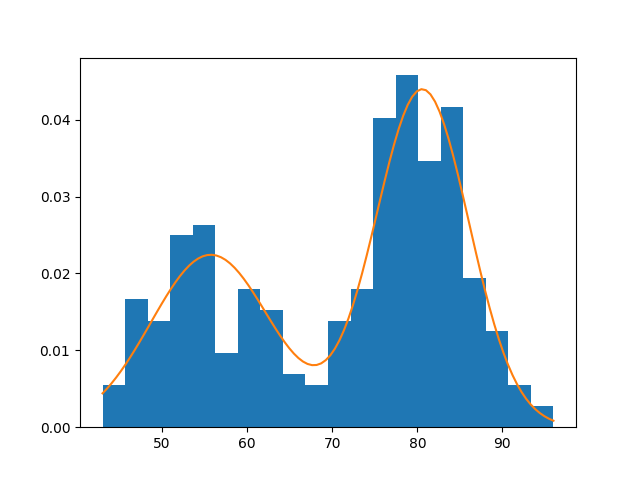
\includegraphics[width=\textwidth]{../code/q2/data_hist_k2.png}
         \caption{K=2}
         \label{fig:k=2}
     \end{subfigure}
     \hfill
     \begin{subfigure}[b]{0.3\textwidth}
         \centering
         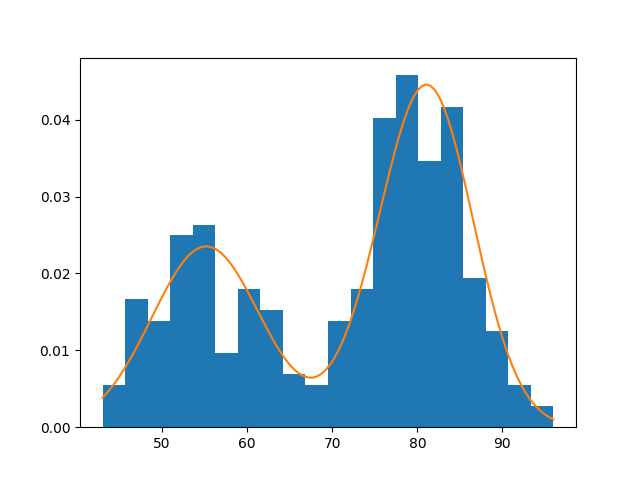
\includegraphics[width=\textwidth]{../code/q2/data_hist_k3.png}
         \caption{K=3}
         \label{fig:k=3}
     \end{subfigure}
     \hfill
     \hfill
     \begin{subfigure}[b]{0.3\textwidth}
         \centering
         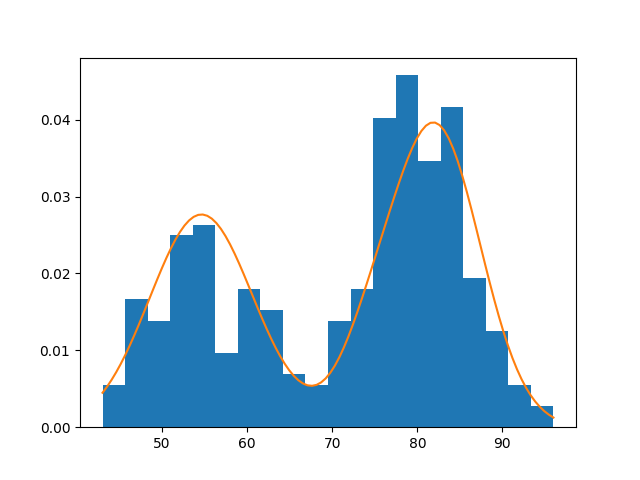
\includegraphics[width=\textwidth]{../code/q2/data_hist_k4.png}
         \caption{K=4}
         \label{fig:k=4}
     \end{subfigure}
     \hfill
     \begin{subfigure}[b]{0.3\textwidth}
         \centering
         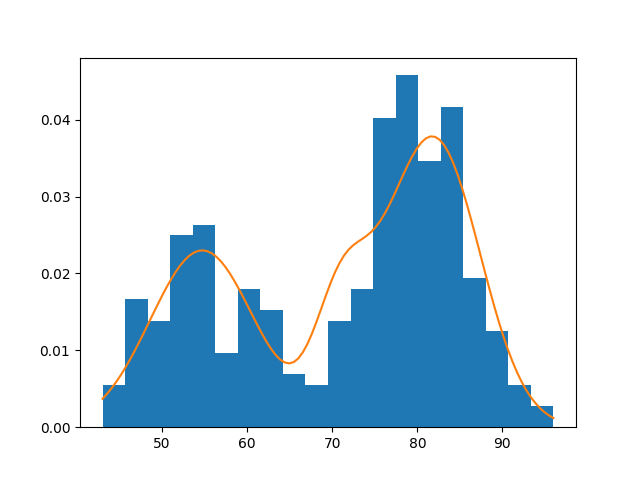
\includegraphics[width=\textwidth]{../code/q2/data_hist_k5.png}
         \caption{K=5}
         \label{fig:k=5}
     \end{subfigure}
     % \hfill
     % \begin{subfigure}[b]{0.3\textwidth}
     %     \centering
     %     \includegraphics[width=\textwidth]{../code/regular_loc_scale_plots/galaxies_hist_k_9.png}
     %     \caption{K=}
     %     \label{fig:Reg_loc_scale}
     % \end{subfigure}
        \caption{Estimated density using Gibbs sampled $\mu$s and $\sigma^2$'s and the stationary distribution from the largest eigenvector.
        I did not have time to figure out how python can plot the credible intervals, although I have all samples so it shouldn't be hard.}
        \label{fig:K_components}
\end{figure}


